\section{Identification de solutions}

Au laboratoire, Enzo a trouvé un flacon sans étiquette, qui contient une solution incolore. 

\begin{center}
	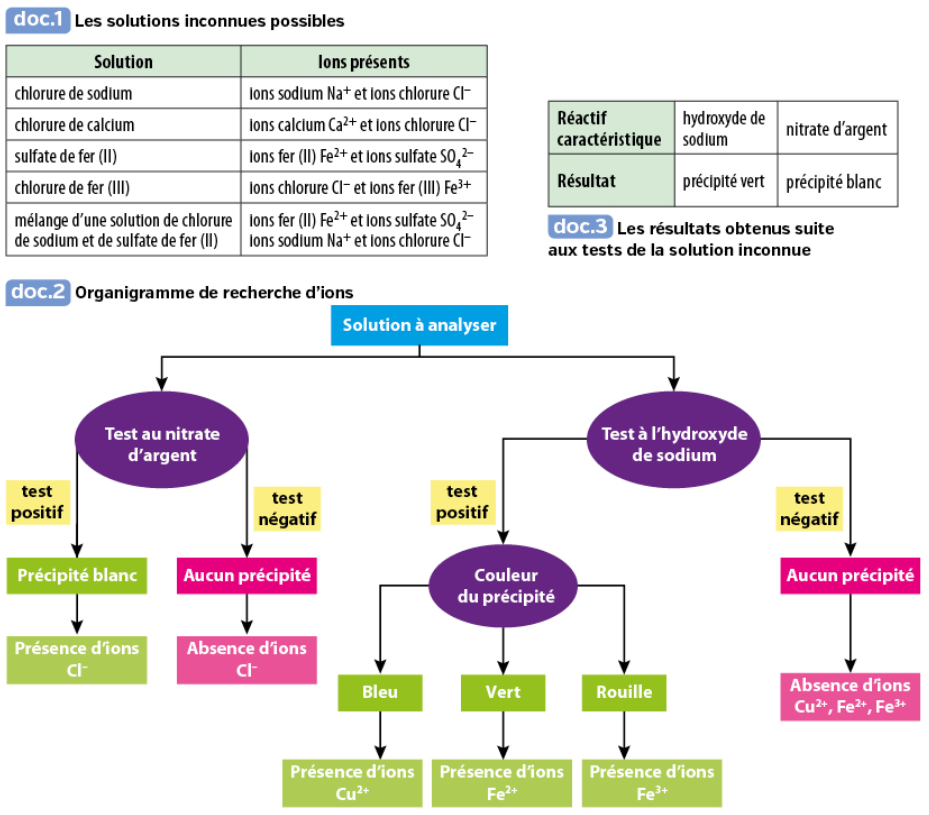
\includegraphics[scale=0.6]{img/docs}
\end{center}

\begin{questions}
	\question La solution inconnue est l'une de celles présentes dans le doc. 1. Quels tests doit-il faire pour l'identifier ? Décrire le protocole expérimental.
	\begin{solution}
		Pour identifier la solution inconnue, Enzo devra :
		\begin{itemize}
			\item verser quelques millilitres de la solution dans deux tubes à essais;
			\item ajouter quelques goutes de nitrate d'argent dans le premier tube;
			\item ajouter quelques goutes de soude dans le second tube;
			\item observer les résultats.
		\end{itemize}
	\end{solution}
	
	\question Représenter un de ces tests à l'aide d'un schéma.
	\begin{solution}
		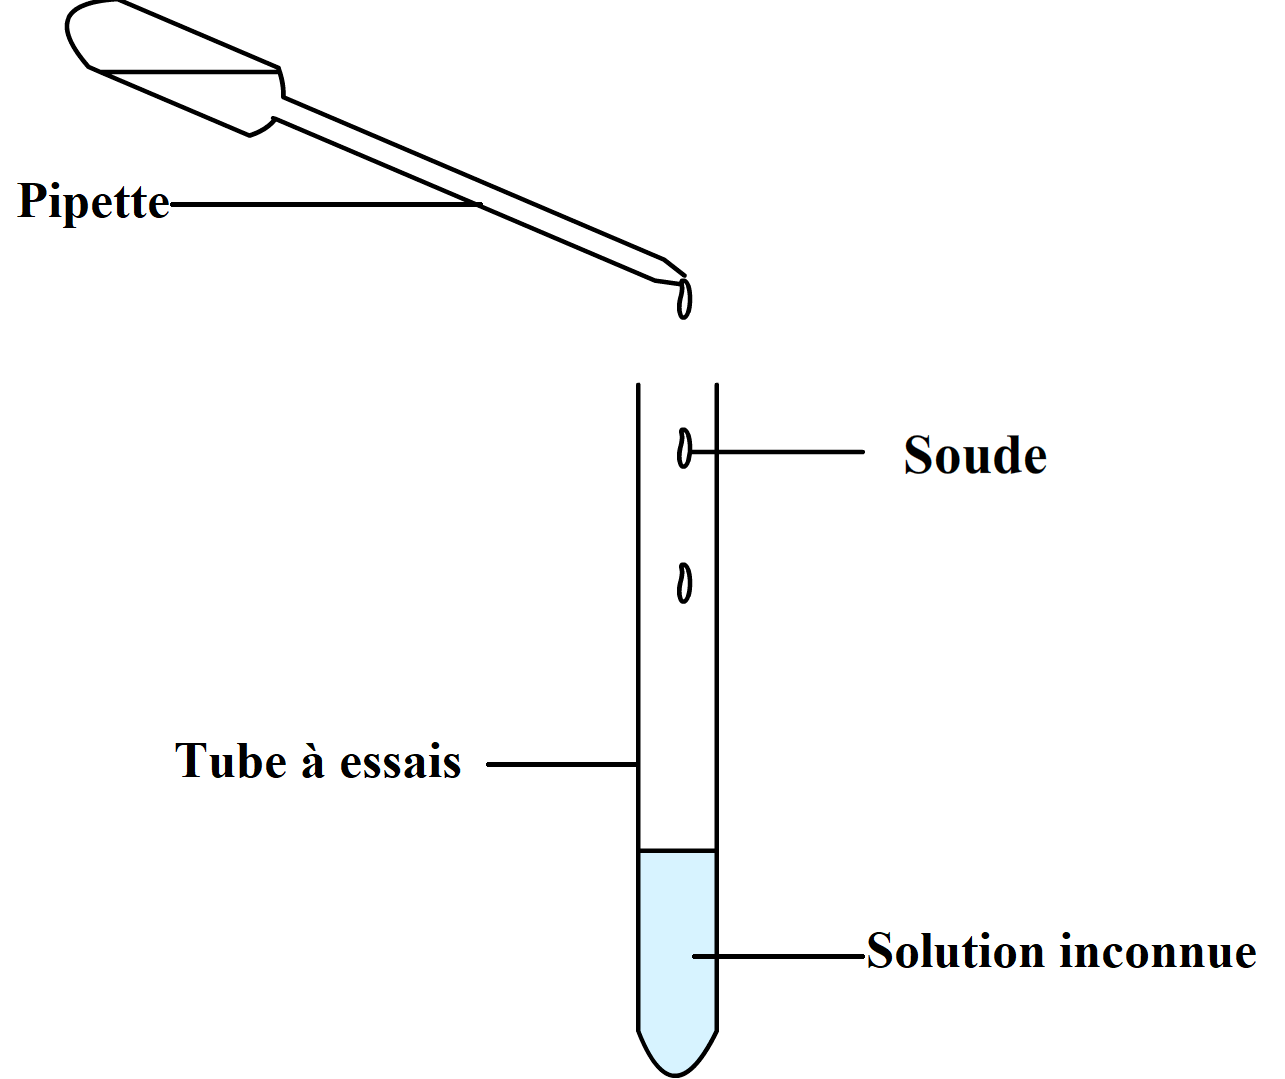
\includegraphics[scale=0.2]{img/ajout-soude}
	\end{solution}
	
	\question D'après les résultats obtenus présentés dans le doc. 3, quels ions ont été identifiés par les tests ? 
	\begin{solution}
		La solution à réagit avec la soude en formant un précipité vert et avec le nitrate d'argent en formant un précipité blanc. Elle contient donc des ions Fer II ($Fe^{2+}$)et Chlorure ($Cl^-$).
	\end{solution}
	
	\question Quelle est la solution contenue dans le flacon ?
	\begin{solution}
		La solution contenue dans le flacon est donc un mélange de cholrure de sodium et de sulfate de fer (II).
	\end{solution}
	
	\question Détailler la composition de chacun des ions présents dans la solution. (nombre de protons, nombre d'électrons, nombre de charges).
	\begin{solution}
		Le numéro atomique de l'atome de fer est 26, l'ion fer II contient donc 26 protons, 24 électrons et 2 charges positives.
		
		Le numéro atomique de l'atome de chlore est 17, l'ion chlorure contient donc 17 protons, 18 électrons et 1 charge négative.
	\end{solution}
	
\end{questions}